\documentclass{standalone}
\usepackage{tikz}
\usetikzlibrary{patterns, positioning}
\usepackage[sfdefault]{ClearSans} %% option 'sfdefault' activates Clear Sans as the default text font
\usepackage[T1]{fontenc}

\begin{document}
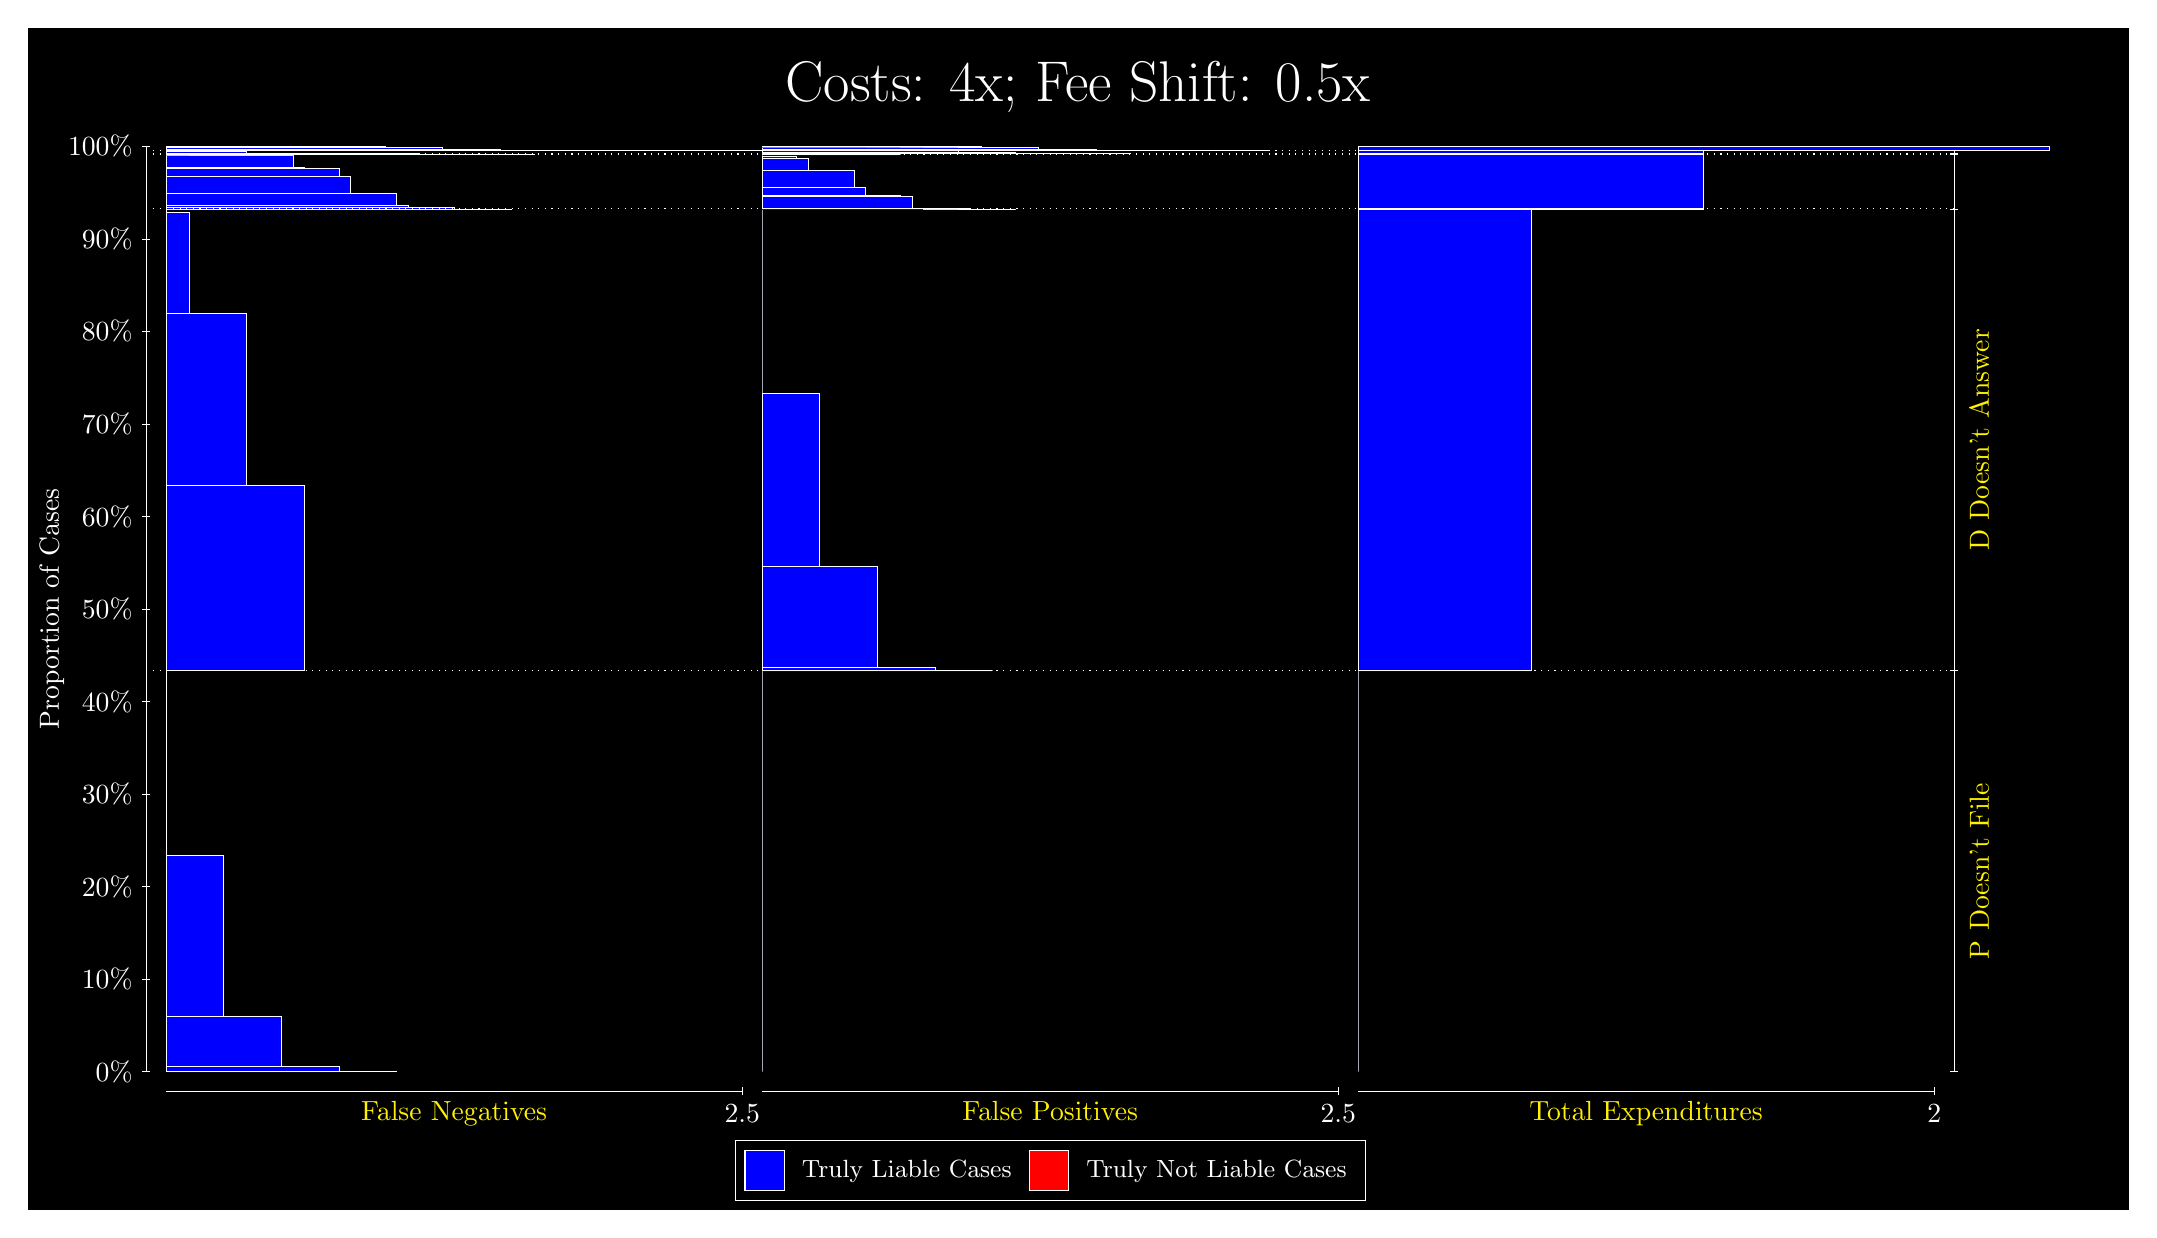
\begin{tikzpicture}
\draw[fill=black] (0,0) rectangle (26.667,15);
\draw[text=white] (0,13.5) rectangle (26.667,15) node[midway] {\huge Costs: 4x; Fee Shift: 0.5x};
\draw[white, very thin] (1.5,1.75) -- (1.5,13.5);
\node[rotate=90, text=white, anchor=center] at (0.3, 7.625) {Proportion of Cases};
\draw[white, very thin] (1.45,1.75) -- (1.55,1.75);
\node[text=white, anchor=east] at (1.45, 1.75) {0\%};
\draw[white, very thin] (1.45,2.925) -- (1.55,2.925);
\node[text=white, anchor=east] at (1.45, 2.925) {10\%};
\draw[white, very thin] (1.45,4.1) -- (1.55,4.1);
\node[text=white, anchor=east] at (1.45, 4.1) {20\%};
\draw[white, very thin] (1.45,5.275) -- (1.55,5.275);
\node[text=white, anchor=east] at (1.45, 5.275) {30\%};
\draw[white, very thin] (1.45,6.45) -- (1.55,6.45);
\node[text=white, anchor=east] at (1.45, 6.45) {40\%};
\draw[white, very thin] (1.45,7.625) -- (1.55,7.625);
\node[text=white, anchor=east] at (1.45, 7.625) {50\%};
\draw[white, very thin] (1.45,8.8) -- (1.55,8.8);
\node[text=white, anchor=east] at (1.45, 8.8) {60\%};
\draw[white, very thin] (1.45,9.975) -- (1.55,9.975);
\node[text=white, anchor=east] at (1.45, 9.975) {70\%};
\draw[white, very thin] (1.45,11.15) -- (1.55,11.15);
\node[text=white, anchor=east] at (1.45, 11.15) {80\%};
\draw[white, very thin] (1.45,12.325) -- (1.55,12.325);
\node[text=white, anchor=east] at (1.45, 12.325) {90\%};
\draw[white, very thin] (1.45,13.5) -- (1.55,13.5);
\node[text=white, anchor=east] at (1.45, 13.5) {100\%};

\draw[white, very thin] (24.457,1.75) -- (24.457,13.5);
\draw[white, very thin] (24.407,1.75) -- (24.507,1.75);
\node[anchor=west] at (24.407, 1.75) {};
\draw[white, very thin] (24.407,6.841) -- (24.507,6.841);
\node[anchor=west] at (24.407, 6.841) {};
\draw[white, very thin] (24.407,12.706) -- (24.507,12.706);
\node[anchor=west] at (24.407, 12.706) {};
\draw[white, very thin] (24.407,13.394) -- (24.507,13.394);
\node[anchor=west] at (24.407, 13.394) {};
\draw[white, very thin] (24.407,13.413) -- (24.507,13.413);
\node[anchor=west] at (24.407, 13.413) {};
\draw[white, very thin] (24.407,13.449) -- (24.507,13.449);
\node[anchor=west] at (24.407, 13.449) {};
\draw[white, very thin] (24.407,13.5) -- (24.507,13.5);
\node[anchor=west] at (24.407, 13.5) {};

\draw[white, very thin, fill=blue] (1.75,1.75) rectangle (4.6775,1.7506);
\draw[white, very thin, fill=blue] (1.75,1.7506) rectangle (3.9457,1.8155);
\draw[white, very thin, fill=blue] (1.75,1.8155) rectangle (3.2138,2.4558);
\draw[white, very thin, fill=blue] (1.75,2.4558) rectangle (2.4819,4.4941);
\draw[white, very thin, fill=red] (1.75,4.4941) rectangle (1.75,4.4941);
\draw[white, very thin, fill=blue] (1.75,4.4941) rectangle (1.75,6.841);
\draw[white, very thin, fill=blue] (1.75,6.841) rectangle (3.5065,9.1893);
\draw[white, very thin, fill=blue] (1.75,9.1893) rectangle (2.7746,11.386);
\draw[white, very thin, fill=blue] (1.75,11.386) rectangle (2.0428,12.662);
\draw[white, very thin, fill=red] (1.75,12.662) rectangle (1.75,12.662);
\draw[white, very thin, fill=blue] (1.75,12.662) rectangle (1.75,12.706);
\draw[white, very thin, fill=blue] (1.75,12.706) rectangle (6.1413,12.706);
\draw[white, very thin, fill=blue] (1.75,12.706) rectangle (5.5558,12.706);
\draw[white, very thin, fill=blue] (1.75,12.706) rectangle (5.4094,12.728);
\draw[white, very thin, fill=blue] (1.75,12.728) rectangle (4.9703,12.728);
\draw[white, very thin, fill=blue] (1.75,12.728) rectangle (4.8239,12.75);
\draw[white, very thin, fill=blue] (1.75,12.75) rectangle (4.6775,12.898);
\draw[white, very thin, fill=blue] (1.75,12.898) rectangle (4.2384,12.906);
\draw[white, very thin, fill=blue] (1.75,12.906) rectangle (4.092,13.125);
\draw[white, very thin, fill=blue] (1.75,13.125) rectangle (3.9457,13.226);
\draw[white, very thin, fill=blue] (1.75,13.226) rectangle (3.5065,13.231);
\draw[white, very thin, fill=blue] (1.75,13.231) rectangle (3.3602,13.39);
\draw[white, very thin, fill=blue] (1.75,13.39) rectangle (3.2138,13.392);
\draw[white, very thin, fill=blue] (1.75,13.392) rectangle (2.7746,13.392);
\draw[white, very thin, fill=blue] (1.75,13.392) rectangle (2.6283,13.394);
\draw[white, very thin, fill=blue] (1.75,13.394) rectangle (2.0428,13.394);
\draw[white, very thin, fill=red] (1.75,13.394) rectangle (1.75,13.394);
\draw[white, very thin, fill=blue] (1.75,13.394) rectangle (6.4341,13.394);
\draw[white, very thin, fill=blue] (1.75,13.394) rectangle (5.7022,13.398);
\draw[white, very thin, fill=blue] (1.75,13.398) rectangle (4.9703,13.408);
\draw[white, very thin, fill=blue] (1.75,13.408) rectangle (4.2384,13.413);
\draw[white, very thin, fill=blue] (1.75,13.413) rectangle (3.5065,13.413);
\draw[white, very thin, fill=red] (1.75,13.413) rectangle (1.75,13.413);
\draw[white, very thin, fill=blue] (1.75,13.413) rectangle (3.5065,13.413);
\draw[white, very thin, fill=blue] (1.75,13.413) rectangle (2.7746,13.433);
\draw[white, very thin, fill=blue] (1.75,13.433) rectangle (2.0428,13.449);
\draw[white, very thin, fill=red] (1.75,13.449) rectangle (1.75,13.449);
\draw[white, very thin, fill=blue] (1.75,13.449) rectangle (1.75,13.449);
\draw[white, very thin, fill=blue] (1.75,13.449) rectangle (9.9471,13.449);
\draw[white, very thin, fill=blue] (1.75,13.449) rectangle (9.2152,13.449);
\draw[white, very thin, fill=blue] (1.75,13.449) rectangle (8.4834,13.45);
\draw[white, very thin, fill=blue] (1.75,13.45) rectangle (7.7515,13.453);
\draw[white, very thin, fill=blue] (1.75,13.453) rectangle (7.4587,13.453);
\draw[white, very thin, fill=blue] (1.75,13.453) rectangle (7.0196,13.453);
\draw[white, very thin, fill=blue] (1.75,13.453) rectangle (6.7268,13.454);
\draw[white, very thin, fill=blue] (1.75,13.454) rectangle (6.2877,13.454);
\draw[white, very thin, fill=blue] (1.75,13.454) rectangle (5.9949,13.462);
\draw[white, very thin, fill=blue] (1.75,13.462) rectangle (5.2631,13.487);
\draw[white, very thin, fill=blue] (1.75,13.487) rectangle (4.5312,13.499);
\draw[white, very thin, fill=blue] (1.75,13.499) rectangle (3.7993,13.5);
\draw[white, very thin, fill=blue] (1.75,13.5) rectangle (3.0674,13.5);
\draw[white, very thin, fill=blue] (1.75,13.5) rectangle (2.3355,13.5);
\draw[white, very thin, fill=red] (1.75,13.5) rectangle (1.75,13.5);
\draw[white, very thin, fill=red] (9.3189,1.75) rectangle (9.3189,1.75);
\draw[white, very thin, fill=blue] (9.3189,1.75) rectangle (9.3189,6.841);
\draw[white, very thin, fill=red] (9.3189,6.841) rectangle (12.246,6.841);
\draw[white, very thin, fill=blue] (9.3189,6.841) rectangle (12.246,6.841);
\draw[white, very thin, fill=blue] (9.3189,6.841) rectangle (11.515,6.8852);
\draw[white, very thin, fill=blue] (9.3189,6.8852) rectangle (10.783,8.1606);
\draw[white, very thin, fill=blue] (9.3189,8.1606) rectangle (10.051,10.358);
\draw[white, very thin, fill=blue] (9.3189,10.358) rectangle (9.3189,12.706);
\draw[white, very thin, fill=red] (9.3189,12.706) rectangle (12.539,12.706);
\draw[white, very thin, fill=blue] (9.3189,12.706) rectangle (12.539,12.706);
\draw[white, very thin, fill=red] (9.3189,12.706) rectangle (11.954,12.706);
\draw[white, very thin, fill=blue] (9.3189,12.706) rectangle (11.954,12.708);
\draw[white, very thin, fill=blue] (9.3189,12.708) rectangle (11.807,12.708);
\draw[white, very thin, fill=red] (9.3189,12.708) rectangle (11.368,12.708);
\draw[white, very thin, fill=blue] (9.3189,12.708) rectangle (11.368,12.709);
\draw[white, very thin, fill=blue] (9.3189,12.709) rectangle (11.222,12.869);
\draw[white, very thin, fill=blue] (9.3189,12.869) rectangle (11.075,12.873);
\draw[white, very thin, fill=blue] (9.3189,12.873) rectangle (10.636,12.975);
\draw[white, very thin, fill=blue] (9.3189,12.975) rectangle (10.49,13.194);
\draw[white, very thin, fill=blue] (9.3189,13.194) rectangle (10.344,13.202);
\draw[white, very thin, fill=blue] (9.3189,13.202) rectangle (9.9044,13.349);
\draw[white, very thin, fill=blue] (9.3189,13.349) rectangle (9.758,13.372);
\draw[white, very thin, fill=blue] (9.3189,13.372) rectangle (9.6116,13.372);
\draw[white, very thin, fill=blue] (9.3189,13.372) rectangle (9.3189,13.394);
\draw[white, very thin, fill=red] (9.3189,13.394) rectangle (11.075,13.394);
\draw[white, very thin, fill=blue] (9.3189,13.394) rectangle (11.075,13.394);
\draw[white, very thin, fill=blue] (9.3189,13.394) rectangle (10.344,13.398);
\draw[white, very thin, fill=blue] (9.3189,13.398) rectangle (9.6116,13.409);
\draw[white, very thin, fill=blue] (9.3189,13.409) rectangle (9.3189,13.413);
\draw[white, very thin, fill=red] (9.3189,13.413) rectangle (14.003,13.413);
\draw[white, very thin, fill=blue] (9.3189,13.413) rectangle (14.003,13.413);
\draw[white, very thin, fill=blue] (9.3189,13.413) rectangle (13.271,13.413);
\draw[white, very thin, fill=blue] (9.3189,13.413) rectangle (12.539,13.429);
\draw[white, very thin, fill=blue] (9.3189,13.429) rectangle (11.807,13.449);
\draw[white, very thin, fill=blue] (9.3189,13.449) rectangle (11.075,13.449);
\draw[white, very thin, fill=red] (9.3189,13.449) rectangle (15.759,13.449);
\draw[white, very thin, fill=blue] (9.3189,13.449) rectangle (15.759,13.449);
\draw[white, very thin, fill=blue] (9.3189,13.449) rectangle (15.028,13.449);
\draw[white, very thin, fill=red] (9.3189,13.449) rectangle (15.028,13.449);
\draw[white, very thin, fill=blue] (9.3189,13.449) rectangle (15.028,13.449);
\draw[white, very thin, fill=blue] (9.3189,13.449) rectangle (14.296,13.45);
\draw[white, very thin, fill=red] (9.3189,13.45) rectangle (14.296,13.45);
\draw[white, very thin, fill=blue] (9.3189,13.45) rectangle (14.296,13.45);
\draw[white, very thin, fill=blue] (9.3189,13.45) rectangle (13.564,13.453);
\draw[white, very thin, fill=red] (9.3189,13.453) rectangle (13.564,13.453);
\draw[white, very thin, fill=blue] (9.3189,13.453) rectangle (13.564,13.462);
\draw[white, very thin, fill=blue] (9.3189,13.462) rectangle (12.832,13.462);
\draw[white, very thin, fill=blue] (9.3189,13.462) rectangle (12.832,13.487);
\draw[white, very thin, fill=blue] (9.3189,13.487) rectangle (12.1,13.496);
\draw[white, very thin, fill=red] (9.3189,13.496) rectangle (11.807,13.496);
\draw[white, very thin, fill=blue] (9.3189,13.496) rectangle (11.807,13.496);
\draw[white, very thin, fill=blue] (9.3189,13.496) rectangle (11.368,13.496);
\draw[white, very thin, fill=red] (9.3189,13.496) rectangle (11.075,13.496);
\draw[white, very thin, fill=blue] (9.3189,13.496) rectangle (11.075,13.496);
\draw[white, very thin, fill=blue] (9.3189,13.496) rectangle (10.636,13.496);
\draw[white, very thin, fill=blue] (9.3189,13.496) rectangle (10.344,13.499);
\draw[white, very thin, fill=blue] (9.3189,13.499) rectangle (9.6116,13.5);
\draw[white, very thin, fill=blue] (9.3189,13.5) rectangle (9.3189,13.5);
\draw[white, very thin, fill=red] (16.888,1.75) rectangle (16.888,1.75);
\draw[white, very thin, fill=blue] (16.888,1.75) rectangle (16.888,6.841);
\draw[white, very thin, fill=red] (16.888,6.841) rectangle (19.083,6.841);
\draw[white, very thin, fill=blue] (16.888,6.841) rectangle (19.083,12.706);
\draw[white, very thin, fill=red] (16.888,12.706) rectangle (21.279,12.706);
\draw[white, very thin, fill=blue] (16.888,12.706) rectangle (21.279,12.719);
\draw[white, very thin, fill=red] (16.888,12.719) rectangle (21.279,12.719);
\draw[white, very thin, fill=blue] (16.888,12.719) rectangle (21.279,13.394);
\draw[white, very thin, fill=red] (16.888,13.394) rectangle (21.279,13.394);
\draw[white, very thin, fill=blue] (16.888,13.394) rectangle (21.279,13.413);
\draw[white, very thin, fill=red] (16.888,13.413) rectangle (21.279,13.413);
\draw[white, very thin, fill=blue] (16.888,13.413) rectangle (21.279,13.449);
\draw[white, very thin, fill=red] (16.888,13.449) rectangle (25.67,13.449);
\draw[white, very thin, fill=blue] (16.888,13.449) rectangle (25.67,13.453);
\draw[white, very thin, fill=red] (16.888,13.453) rectangle (25.67,13.453);
\draw[white, very thin, fill=blue] (16.888,13.453) rectangle (25.67,13.5);
\draw[white, dotted] (1.5,6.841) -- (24.457,6.841);
\draw[white, dotted] (1.5,12.706) -- (24.457,12.706);
\draw[white, dotted] (1.5,13.394) -- (24.457,13.394);
\draw[white, dotted] (1.5,13.413) -- (24.457,13.413);
\draw[white, dotted] (1.5,13.449) -- (24.457,13.449);
\draw[white, very thin] (1.75,1.5) -- (9.0689,1.5);
\node[text=yellow, anchor=north] at (5.4094, 1.5) {False Negatives};
\draw[white, very thin] (9.0689,1.45) -- (9.0689,1.55);
\node[text=white, anchor=north] at (9.0689, 1.45) {2.5};

\draw[white, very thin] (9.3189,1.5) -- (16.638,1.5);
\node[text=yellow, anchor=north] at (12.978, 1.5) {False Positives};
\draw[white, very thin] (16.638,1.45) -- (16.638,1.55);
\node[text=white, anchor=north] at (16.638, 1.45) {2.5};

\draw[white, very thin] (16.888,1.5) -- (24.207,1.5);
\node[text=yellow, anchor=north] at (20.547, 1.5) {Total Expenditures};
\draw[white, very thin] (24.207,1.45) -- (24.207,1.55);
\node[text=white, anchor=north] at (24.207, 1.45) {2};

\node[text=yellow, centered, rotate=90] at (24.777, 4.2955) {P Doesn't File};
\node[text=yellow, centered, rotate=90] at (24.777, 9.7735) {D Doesn't Answer};





\draw (12.978300999999998,1.5) node[draw=none] (baseCoordinate) {};
\begin{scope}[align=center]
        \matrix[scale=0.5, draw=white, below=0.5cm of baseCoordinate, nodes={draw}, column sep=0.1cm]{
            \node[rectangle, draw, minimum width=0.5cm, minimum height=0.5cm, fill=blue] {}; &
            \node[draw=none, font=\small, text=white] (B) {Truly Liable Cases}; &
            \node[rectangle, draw, minimum width=0.5cm, minimum height=0.5cm, fill=red] {}; &
            \node[draw=none, font=\small, text=white] (B) {Truly Not Liable Cases}; \\
            };
\end{scope}

\end{tikzpicture}
\end{document}